\documentclass{scrarticle}
\usepackage[utf8]{inputenc}
\usepackage{graphicx}
\usepackage{float}
\usepackage[T1]{fontenc}
\usepackage{listings}

\title{SpaceWalk The Game}
\author{Péter Bence, Vasánszky Milán, Székely katalin, Tóth Balázs}
\date{October 2022}

\begin{document}

\maketitle

\tableofcontents

\section{Alapinformációk} 
Ez a specifikáció egy szöveges, szerepjátékos űrkalandjátékhoz készült. A játék- ban mozoghatsz szobáról szobára, gyűjthetsz tárgyakat és új utakat nyithatsz meg a játék világának felfedezéséhez. Találkozhatsz és interakcióba léphetsz NPC-kkel. A program a felhasználótól vár egyszerűbb parancsokat, amelyeket később eseményként megjelenít. A történet X mélységű. Az alkalmazás a felhasználó által adott helytelen bemenetre hibaüzenettel válaszol.

\section{Történetvázlat}
Az év 2094. A mesterséges intelligencia teljes mértékben átvette az irányítást a Föld nevezetű bolygó felett 30 évvel ezelőtt. De nem úgy ahogy gondolod kedves PLAYERNAME. 2064-ben kifejlesztették az Oázis AI-t, ami egyedül azt a cél szolgálja, hogy az emberek kényelemben éljenek. A tökéletes utópisztikus világ, ahol az emberek azért jönnek a Földre, hogy jól érezzék magukat, azzal foglalkozzanak, amivel csak akarnak, és akkor, amikor akarnak. Minden unalmas és monoton feladat elvégzését átvették a robotok és az OAI. Ebbe beletartozik a teljesen automatikus házvezetés, takarítás, bevásárlás, és még a főzés is. Nem kevés következménnyel járt ez az átállás. Beolvasztották az összes fegyvert, megszüntették az autókat, és csak is mindenki buszokkal, vagy kijelölt szállítási eszközzel közlekedhet. A 2045-ös jégkorszak után nagymértékben megcsappant a Föld lakossága. A tervezett 9,44 milliárd ember helyett kevesebb, mint 1 milliárd maradt.

\section{Használati esetek}
\begin{table}[H] \centering
    \caption{Használati esetek}\label{tab:usecasetable}
    \begin{tabular}{@{}ll@{}}
        \emph{Eset} & \emph{Leiras}\\ \hline
        Move         & Mozgas szobarol szobara\\
        Search room  & Kutasd at a szobat, itemek es NPC-k utan\\
        Pick up item & Vegyed fel a talalt targyat\\
        Interact with NPC & Beszelj a talalt NPC-vel\\
        Accept mission & Fogadd el az NPC kuldeteset
    \end{tabular}
\end{table}

\graphicspath{{../Planning/}}
\begin{figure}[H]\centering
    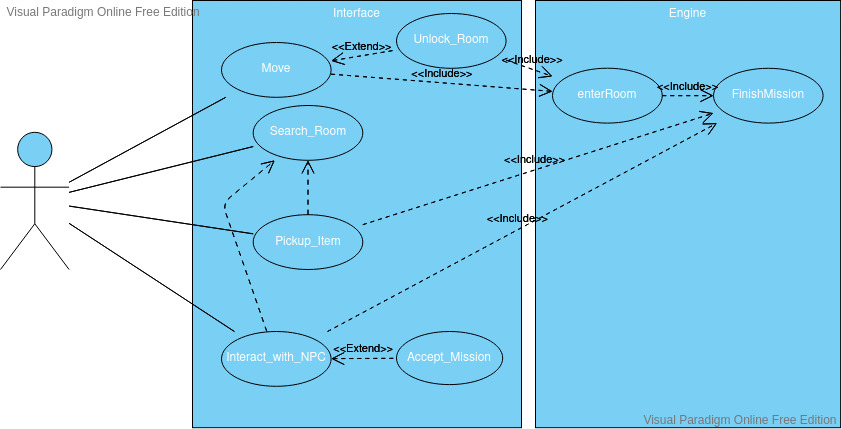
\includegraphics[width=1.0\columnwidth]{Functional_UseCase.jpg}
    \caption{Functional Use Cases}\label{fig:1}
\end{figure}

\section{Struktura}
\begin{figure}[H]
    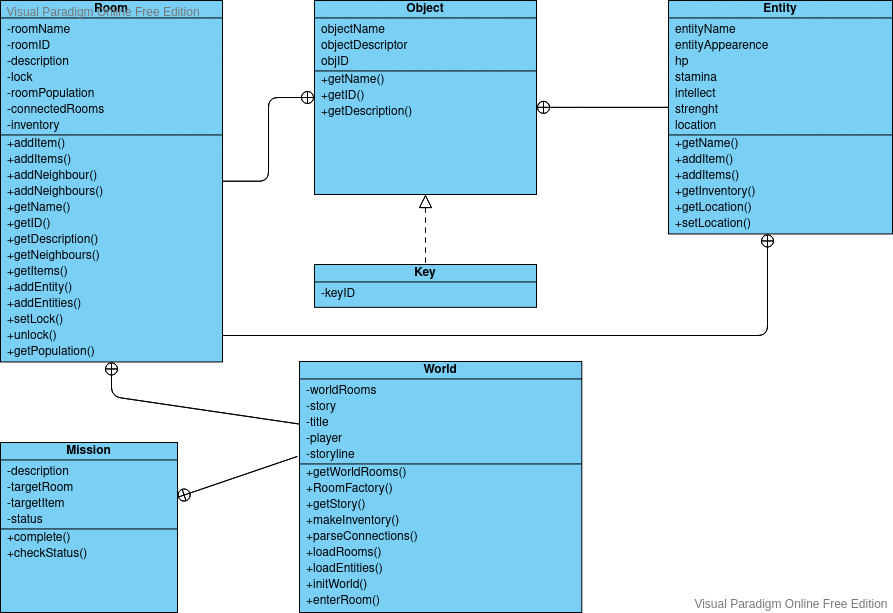
\includegraphics[width=1.0\columnwidth]{Class_Architecture.jpg}
    \caption{Class Architecture}\label{fig:2}
\end{figure}

\begin{figure}[H]
    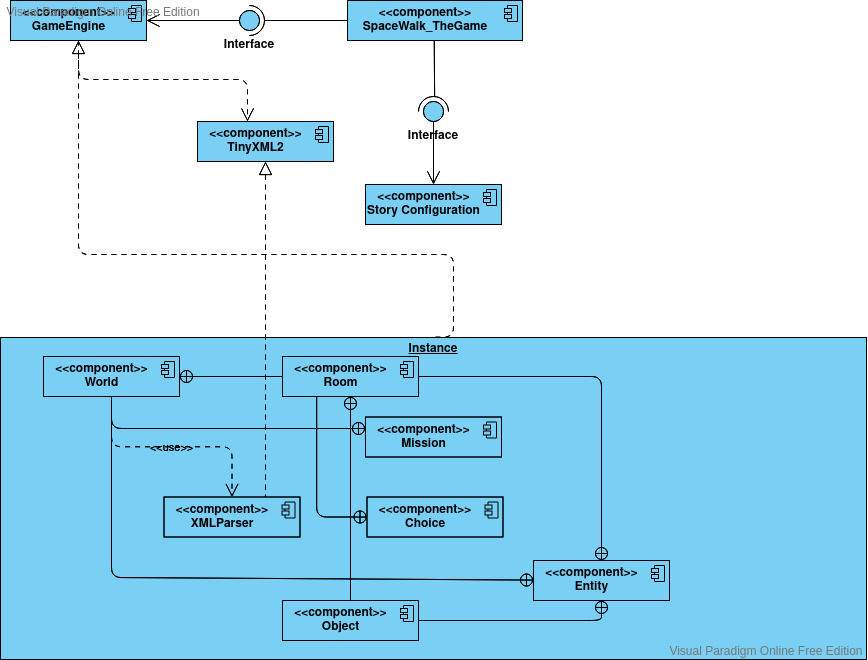
\includegraphics[width=1.0\columnwidth]{Component_Connection.jpg}
    \caption{Component connection}\label{fig:3}
\end{figure}

\section{Viselkedes}
\begin{figure}[H]
    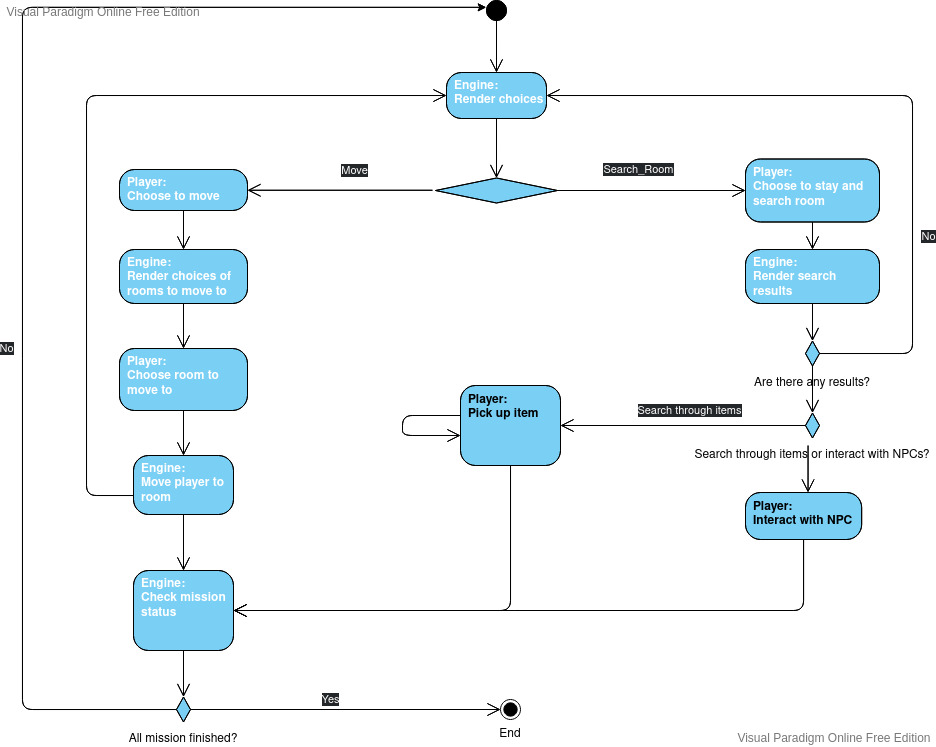
\includegraphics[width=1.0\columnwidth]{GameLoop_ActivityDiagram.jpg}
    \caption{Gameloop Activity Diagram}\label{fig:4}
\end{figure}

\section{Történet tárolási formátuma}
A történetet xml fájlformátumban tároljuk és a TinyXML2 könyvtár segítségével olvassuk be. Az xml fájlformátum lehetővé teszi, hogy a játékvilágot és hozzá tartozó történelem részleteket modulárisan építhessük fel, így szabadon bővíthető lesz, vagy akár egy teljesen más történetet is betölthetünk.

\subsection{XML file felépítése}

\subsubsection{<world>}
A <world> tag-ből szigorúan csak egyet szabad használni, mivel ez fogja tartalmazni a játékvilág összes elemét.

\subsubsection{<title>}
<title> tag-ből megint csak egyet szabad használni, ez tartalmazza a játék címét. Ez a tag a <world> tagnek egy gyereke.

\subsubsection{<room>}
A <room> tag segítségével tölthetjük meg szobákkal a világot, ebből a tagből akármennyit lehet használi, de szigorúan a <world> tag-en belül.

\subsubsection{<name>}
A <name> tag a <room> nevét adja meg.

\subsubsection{<description>}
A <description> tag-el lehet a szobának a leírását, szobához tartozó storyt megadni.

\subsubsection{<id>}
Az <id> tag egyértelműen a szoba azonosítója, ami segít az egyszerű azonosításban, a kulcsokkal való összekötéssel és a szomszéd szobák megadásában.

\subsubsection{<inventory>}
A szobában megtalálható tárgyakat foglalja magába az <inventory> tag, amiből szobánként egy van.

\subsubsection{<object>}
Az <object> tageket az <inventory> tageken belülre kell helyezni, mivel ezzel tudjuk konkrétan megadni egy szobában található tárgynak a tulajdonságait.

\subsubsection{<name>}
Egy tárgynak is van megnevezése, ezért az <object>-en belül is kell használni a name taget.

\subsubsection{<description>}
A tárgyak kinézetét, felhasználási módját a leírás - description - tag-el lehet megadni.

\subsubsection{<id>}
A tárgyakat nehéz lenne csak név és leírás alapján beazonosítani programozási szemszögből így az id tagben megadott id-vel könnyen be lehet azonosítani.

\subsubsection{<entity>}
A szobákban létező NPC-ket az entity tag-el lehet megadni. Az entity-knek is van nevük, a név megadásához az eddig már többször elhangzott <name> tag-el lehet megadni. Az entity-knek is van <inventory>-juk, amiben ugyan úgy lehet megadni a tárgyakat - <object> -, mint a szobáknak.

\subsubsection{<missions>}
Ez az új tag a <world>-tag gyereke, a storyhoz tartózó küldetések megadására szolgál.

\subsubsection{<mission>}
A mission tag-en belül meg kell adni a küldetés leírását <description>-nel adható meg a küldetés leírása. A küldtés célját a <targetRoom> és a <targetItem> tag-el adhatjuk meg, ezeknek a tageknek a szoba vagy tárgy azonosítóját kell tartalmazniuk.

\subsection{Példa az xml story fájl elkészítéséhez}
\lstinputlisting{../test_story.xml}

\end{document}